\documentclass{article}
\usepackage{qilin}
\tikzstyle{process} = [rectangle, rounded corners, minimum width=1.5cm, minimum height=0.5cm,align=center, draw=black, fill=gray!30, auto]
\title{MAT257: Real Analysis II}
\author{QiLin Xue}
\date{Fall 2021}
\usepackage{mathrsfs}
\usetikzlibrary{arrows}
\usepackage{stmaryrd}

\begin{document}

\maketitle
\tableofcontents
\newpage
\section{Differentiation}
\subsection{Inverse Function Theorem}
\begin{theorem}
    Suppose that $f:\mathbb{R}^n \rightarrow \mathbb{R}^n$ is continuously differentiable in an open set containing $a$ and $\det f'(a) \neq 0$. Then there is an open set $V$ containing $a$ and an open set $W$ containing $f(a)$ such that $f:V\rightarrow W$ has a continuous inverse $f^{-1}:W\rightarrow V$ which is differentiable and for all $y\in W$ satisfies
    \begin{equation}
        (f^{-1})'(y) = [f'(f^{-1}(y))]^{-1}
    \end{equation}
\end{theorem}
\textit{Motivation:} In 1D calculus, if a function has a derivative $f'(x)>0$ at some point $x=a$, then around this point the function is monotone and has an inverse, per the intermediate value theorem. We want something similar for multiple dimensions, however there is no equivalent intermediate value theorem.

We will motivate our proof with the following steps
\begin{enumerate}
    \item Prove the last step, as it is the easiest.
    \item WLOG, make the simplifying assumption that $f'(a) = I$.
    \item Define ``all-scale fidelity'' to describe how vectors in an open neighbourhood around $a$ are \textit{nearly} preserved. Then show that $f$ has all-scale fidelity on some neighbourhood $U$ around $a$. 
    \item Given $y\in W$. We can construct a sequence $(x_i)$ such that $\{f(x_i)\}$ is a Cauchy sequence which converges to $y.$ 
    \item Show that there exists an $x\in V$ such that $f(x)=y,$ by invoking continuity. Said differently, $f|_V: V\rightarrow W$ is onto.
    \item Show that $f|_V: V\rightarrow W$ is injective (1-1).
    \item We have shown that $f^{-1}$ exists. We now need to show that $f^{-1}$ is continuous.
    \item Show that $f^{-1}$ is differentiable at the point $f(a)=b$.
    \item Show that $f^{-1}$ is differentiable at a point near $b$.
    \item Show that $f^{-1}(y)$ is continuously differentiable near $b$.
\end{enumerate}
Let us perform these steps:
\begin{enumerate}
    \item Consider the following setup
    \begin{center}
        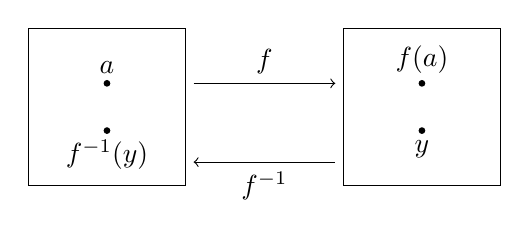
\begin{tikzpicture}
            
            \draw[] (0,0) rectangle (2,2);
            \draw[->] (2.1, 1.3) -- (3.9, 1.3) node[above, midway] {$f$}; 
            \draw[<-] (2.1, 0.3) -- (3.9, 0.3) node[below, midway] {$f^{-1}$}; 

            \draw[] (4,0) rectangle (6,2);

            
            \filldraw[black] (1,1.3) circle (1pt) node[anchor=south]{$a$};
            \filldraw[black] (5,1.3) circle (1pt) node[anchor=south]{$f(a)$};
            \filldraw[black] (1,0.7) circle (1pt) node[anchor=north]{$f^{-1}(y)$};
            \filldraw[black] (5,0.7) circle (1pt) node[anchor=north]{$y$};

        \end{tikzpicture}
    \end{center}
    Recall that $f \circ f^{-1} = I$, so differentiating and applying the chain rule we can write 
    \begin{equation}
        f'(f^{-1}(y)) \cdot (f^{-1})'(y) = I \implies (f^{-1})'(y) = [f'(f^{-1}(y))]^{-1}
    \end{equation}
    \item We are allowed to write $f'(a) = I$ since every invertible matrix is just the identity with a change of basis. More concretely, consider another composition represented below, where $L=f'(a):$
    \begin{center}
        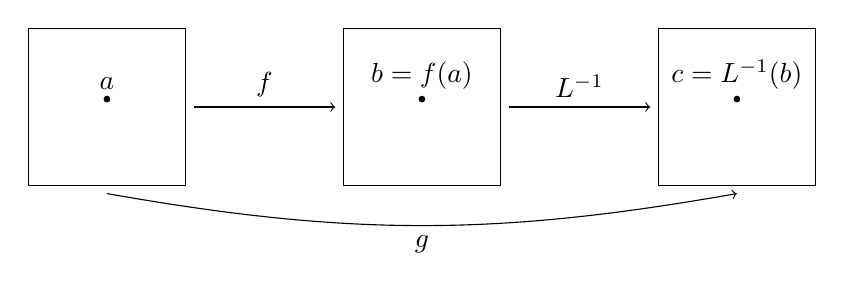
\begin{tikzpicture}
            
            \draw[] (0,0) rectangle (2,2);
            \draw[->] (2.1, 1) -- (3.9, 1) node[above, midway] {$f$}; 
            \draw[->] (6.1, 1) -- (7.9, 1) node[above, midway] {$L^{-1}$}; 

            \draw[] (4,0) rectangle (6,2);
            \draw[] (8,0) rectangle (10,2);

            
            \filldraw[black] (1,1.1) circle (1pt) node[anchor=south]{$a$};
            \filldraw[black] (5,1.1) circle (1pt) node[anchor=south]{$b=f(a)$};
            \filldraw[black] (9,1.1) circle (1pt) node[anchor=south]{$c=L^{-1}(b)$};

            \draw [->,black] (1,-0.1) to [out=-10,in=190] node[below, midway] {$g$} (9,-0.1);

        \end{tikzpicture}
    \end{center}
    By the chain rule, we have $g'(a) = L^{-1} \circ f'(a)$ since $L^{-1}$ is a linear transformation. Note that $f'(a) = L$, so $g'(a) = I$ is the identity.

    If the IFT was true for functions whose differential is $I$, then it's true for $g$, so there exists $g^{-1}$. Also, $f^{-1} = g^{-1} \circ L^{-1}.$ Therefore, if $g^{-1}$ is continuously differentiable, then $f^{-1}$ would also be continuously differentiable. Thus, it is sufficient to only look at the case where the differential is the identity.

    \item Consider a small neighbourhood around $a$. Intuitively, we should expect vectors and the image of the vectors (which need not start at $a$) to look roughly the same.
    
    Specifically, $f$ has \textbf{all-scale-fidelity} on some neighbourhood $U$ of $a$ with \textit{fidelity factor} $\frac{1}{257}.$ This means for all $x_1,x_2 \in U$, we have
    \begin{equation}
        |(x_2-x_1) - (f(x_2)-f(x_1))| \le \frac{1}{257}|x_2-x_1|
    \end{equation}
    \begin{proof}
        From a previous theorem, if we have a function $g:\mathbb{R}^n\rightarrow\mathbb{R}^n$ whose derivative $|g'| < M$ is bounded in some open set, then we can write 
        \begin{equation}
            |g(x_1)-g(x_2)| < n^2M|x_1-x_2|.
        \end{equation} 
        Now consider $g(x) = f(x) - x$. The derivative is $g'=f'-I$ so $g'(a)=0.$ Therefore, there exists an open rectangle $U$ of $a$ where we can say $|g'(x)| \le \frac{1}{257n^2}.$

        By the previous theorem, for any $x_1,x_2 \in U$, we have
        \begin{equation}
            |g(x_1)-g(x_2)| \le \frac{1}{257}|x_1-x_2|
        \end{equation}
        However, the LHS is just 
        \begin{align*}
            |g(x_1)-g(x_2)| &= |f(x_1)-x_1-(f(x_2)-x_2)| \\ 
            &= |(x_2-x_1)-(f(x_2)-f(x_1))|
        \end{align*}
    \end{proof}
    \item Given $y\in W$, we wish to find an $x \in V$ such that $f(x)=y$. We will travel this direction in $W$, but we may ``miss'' by a bit. We can then repeat this process, with each step we travel in the direction of $y$.
    
    Put this formally, let $W=B_{r/2}(b).$ Given $y\in W$, we claim that there exists an $x\in B_r(a)$ such that $f(x)=y.$ Indeed,
    \begin{align}
        x_1 &= a+(y-b) \\ 
        x_2 &= x_1+(y-f(x_1)) \\ 
        x_3 &= x_2+(y-f(x_2)) \\ 
        x_n &= x_{n-1} + (y-f(x_{n-1}))
    \end{align}
    But the difference between any two consecutive terms is just the LHS of the all-scale fidelity
    \begin{align}
        |x_n-x_{n-1}| &= |(x_{n-1}-x_{n-2})-(f(x_{n-1}-f(x_{n-2}))| \\ 
        &\le \frac{1}{257}|x_{n-1}-x_{n-2}| \\ 
        &\le \frac{1}{257^{n-1}} |x_1-x_0| \\ 
        &\le \frac{1}{257^{n-1}} | y-b| \\ 
        &\le \frac{1}{257^{n-1}} \frac{r}{2}
    \end{align}
    We now need to show that each $x_i$ is within the ball of radius $r$ around $a$ (since this is only when all-scale fidelity is defined). It can be shown via induction that $|x_n-a| \le r.$

    Finally, we show that $(x_n)$ is a Cauchy-Sequence. We can immediately show this by noting that
    \begin{equation}
        |x_n-x_m| \le \frac{1}{257^m}r
    \end{equation}
    so $(x_n)$ is cauchy.
    \item While we have shown that $f(x_n)$ converges to $y$, we have not yet shown that this is possible, i.e. what if there is a discontinuity? We can invoke the continuity of $f$ to show that there does exist such an $x_n.$ We have
    \begin{equation}
        |f(x_n)-y| = |x_{n+1}-x_n| \le \frac{1}{257^n}\frac{r}{2} \rightarrow 0
    \end{equation}
    so from continuity, there exists an $x$ such that
    \begin{equation}
        |f(x)-y| = \lim_{n\to \infty} |f(x_n)-y|  = 0.
    \end{equation}
    Therefore, $f(x)=y.$ We can now define $V=F^{-1}(W)$ and now 
    \begin{equation}
        F|_V: V\rightarrow W
    \end{equation}
    is onto and 1-1.
    \item We have constructed $x$ in one such way. How do we know that if we use a different procedure, we find a different $x$?
    
    Assume that $f(x_1)=f(x_2)$ where $x_{1,2} \in B_r(a).$ Then by ASF,
    \begin{align}
        |(x_1-x_2)-(f(x_1)-f(x_2))| &\le \frac{1}{257}|x_1-x_2| \\ 
        |x_1-x_2| & \le \frac{1}{257}|x_1-x_2|
    \end{align}
    which is true if and only if $x_1=x_2.$

    \item It might seem that continuity for $f^{-1}$ is cheap. After all, the difference between two vectors in both the input and image space is roughly the same. However, the mistake is written in terms of $|x_1-x_2|$, so this reasoning becomes circular. We need to reformulate the ASF principle such that the mistake is in terms of $|y_1-y_2|.$
    
    To simplify things, let $\alpha=x_1-x_2$ and $\beta=f(x_1)-f(x_2).$ Then ASF says that
    \begin{equation}
        |\alpha-\beta | \le \frac{1}{257}|\alpha|
    \end{equation}
    But $\alpha = \beta + \alpha - \beta$. By the triangle inequality, this becomes
    \begin{align}
        |\alpha-\beta | &\le \frac{1}{257}(|\beta|+|\alpha-\beta|) \\ 
        \frac{256}{257}|\alpha-\beta| &\le \frac{1}{257}|\beta \\ 
        |\alpha-\beta| &\le \frac{1}{256}\beta
    \end{align}
    
    \item Let us first show that $f^{-1}$ is differentiable at the point $b$. We can write 
    \begin{equation}
        f^{-1}(b+h) = f^{-1}(b) + I\cdot h + e(h)
    \end{equation}
    We want to show that $e(h)$ is tiny. We want to rearrange this in a form such that we can apply all scale fidelity. Let $b+h = y_2$ and let $x_2=f^{-1}(y_2).$ Let $b=y_1$ and $a=x_1$, so the above just becomes 
    \begin{equation}
        x_2 = x_1 + y_2-y_1 + e(h)
    \end{equation}
    However the error once rearranged becomes 
    \begin{equation}
        |e(h)| = |(x_2-x_1)-(y_2-y_1)| \le \frac{1}{256}|y_2-y_1|
    \end{equation}
    Since $y_2-y_1=h$, we end up with 
    \begin{equation}
        \frac{|e(h)|}{|h|} \le \frac{1}{256}
    \end{equation}
    Now we have a problem: we want to show that this approaches zero. This condition is not good enough. However, this constant was chosen arbitrarily, so we can make $\frac{|e(h)|}{|h|}$ as small as possible.
    \item Similarly, the choice of $b$ was also arbitrary. If the conditions for the IFT hold at $a$, then they have to hold in an open set near $a$ (due to continuity). Therefore, we can rewrite the entire proof by considering points near $b$ and not just $b$.
    \item To show $f^{-1}$ is continuously differentiable, we can use the chain rule: 
    \begin{equation}
        (f^{-1})'(y) = [f'(f^{-1}(y))]^{-1}
    \end{equation}
    We can conclude that $f^{-1}(y)$ is continuous in $y$ and $f'(x)$ is continuous in $x$. Therefore, $M \mapsto M^{-1}$ is a continuous operation on matrices. Specifically, it is a function that maps $\mathbb{R}^{n^2}\rightarrow \mathbb{R}^{n^2}.$ This is not everywhere defined. But where defined, the inverse is continuous by Cramer's Law. There is an explicit formula for the inverse, so this map is continuous.
\end{enumerate}

\newpage
\section{Integration}
\subsection{Integrability, Measure 0, Content 0, Integrability and Continuity}
\begin{definition}
    $A$ is of measure $0$ means that for $\forall \epsilon > 0$, there exists open (alternatively closed) rectangles $(R_i)_{i=1}^\infty$ such that
    \begin{enumerate}
        \item $A \subset \bigcup R_i$
        \item $\sum \text{vol}(R_i) < \epsilon.$
    \end{enumerate}
\end{definition}
For example, finite \& countable sets, along with $\mathbb{R} \subset \mathbb{R}^2$ are of measure $0$. 
\begin{definition}
    A set $X$ is called \textbf{countably infinite} if there is a surjective function $F$ such that $F: \mathbb{N} \onto X$
\end{definition}
A few facts that follows:
\begin{enumerate}
    \item Finite sets are countable. (Typically, we exclude this from the definition.)
    \item Subsets of countable sets are countable. (Proof: Elements in a countable set can be enumerated. Simply select a new enumeration.)
    \item A finite/countable union of countable sets is countable. If $A_i$ is countable for all $i$, then $\bigcup A_i$ is countable.
    \begin{proof}
        Consider
        \begin{align*}
            A_1:&\quad a_{11}\quad a_{12}\quad a_{13}\quad \cdots \\
            A_2:&\quad a_{21}\quad a_{22}\quad a_{23}\quad \cdots \\ 
            A_3:&\quad a_{31}\quad a_{32}\quad a_{33}\quad \cdots \\ 
        \end{align*}
        To enumerate the union, we look at the diagonals, i.e.
        \begin{equation}
            \bigcup A = \{a_{11}, a_{12}, a_{21}, a_{13}, a_{22}, a_{31}, \dots \}
        \end{equation}
    \end{proof}
    Another fact that immediately follows is that the set of integers is countable, since $\mathbb{Z} = (-\mathbb{N})\cup \{0\} \cup \mathbb{N}$
    \item If $A,B$ are countable, then $A\times B$ is countable.
    \begin{proof}
        We can prove this similar to how a countable union of sets is countable. Alternatively, we can write 
        \begin{equation}
            A\times B = \bigcup_{b\in B} A \times \{b\}
        \end{equation}
        And each set $A\times \{b\}$ is coutnable.
    \end{proof}
    A fact that follows is that the set of rationals is countable, since $\mathbb{Q} \subset \mathbb{Z}\times \mathbb{Z}.$
\end{enumerate}
It may seem a bit suspicious since up to this point, everything is countable. However, there are sets that are uncountable!
\begin{theorem}
    $\mathbb{R}$ is not countable. And hence, irrational numbers are not countable, i.e. there are ``more'' reals than naturals, more irrationals than rationals.
\end{theorem}
\begin{proof}
    Assume that $\mathbb{R}$ is countable, that is $(a_i)$ is an enumeration of the real numbers. Let $x$ be a real number whose $k^\text{th}$ decimal digit is different from the $k^\text{th}$ decimal digit of $a_k$. Note that $x$ cannot be any of the $a_k$s, hence $\{a_k\}\neq \mathbb{R}$.
\end{proof}
We can now state and prove a few statements about measure-$0$.
\begin{enumerate}
    \item If $A$ is measure-$0$ and $B\subset A$, then $B$ is measure-$0$.
    \item A countable union of measure-$0$ sets is measure-$0$.
    \begin{proof}
        Suppose $\forall i$, $A_i$ is of measure $0$, so given $\epsilon > 0$, we can cover $A_i$ with countably many rectangles whose $\sum\text{vols} < \frac{\epsilon}{2^i}$. Take all the rectangles above together, as a countable collection of countable sets, this collection of rectangles is countable, and 
        \begin{equation}
            \sum\text{vols} < \sum_{i=1}^\infty \frac{\epsilon}{2^i} = \epsilon.
        \end{equation} 
        Finally this collection covers
        \begin{equation}
            \bigcup A_i = A
        \end{equation}
        so $A$ is measure-$0$.
    \end{proof}
    Note that we have stated before that $\mathbb{R} \subset \mathbb{R}^2$  
\end{enumerate}
\begin{warning}
    Countable sets are measure-$0$, but the converse is not true! For example, $\mathbb{R}\subset\mathbb{R}^2$ has measure-$0$, but is not countable.
\end{warning}
Another Example: Let $\mathcal{C}$ be the cantor set $\subset [0,1]$ which is uncountable, yet of measure-$0$ in $\mathbb{R}$. Let
\begin{equation}
    \mathcal{C} = \{0.C_1C_2C_3C_4\dots: C_i \in \{0,2\}\}
\end{equation}
$C$ is uncountable for the same reason as $\mathbb{R}$. Define $C_k$ to be the union of $2^k$ intervals of length $\frac{1}{3^k}$. THerefore, 
\begin{equation}
    C \subset C_k
\end{equation}
where $C_k$ itself is a union of intervals of total length $2^k \cdot \frac{1}{3^k} = \left(\frac{2}{3}\right)^k$, which approaches $0$.

Therefore, $C$ is measure-$0$. As an aside, each $C_k$ is compact, so $\mathcal{C} = \cap C_K$ is therefore also compact.
\begin{theorem}
    $[a,b] \subset \mathbb{R}$ is \textit{not} measure $0$. In fact, $R \subset \mathbb{R}^n$ is not measure $0$.
\end{theorem}
\begin{definition}
    $A\subset \mathbb{R}^n$ is said to be of content-$0$ if $\forall \epsilon > 0$ it is contained in a finite union of rectangles whose sum of volumes is smaller than $\epsilon$.
\end{definition}
Note that $\mathbb{Z} \in \mathbb{R}$ is not of content-$0$.
\end{document}